\section{Experiment}\label{sec:method}
\subsection{Method}
To test if our product helps solve our product statement, we wish
to make an experiment that quantitatively evaluates the effectiveness of our
program. 

To do this, we have devised the following experiment:
\begin{figure}[H]
  \centering
  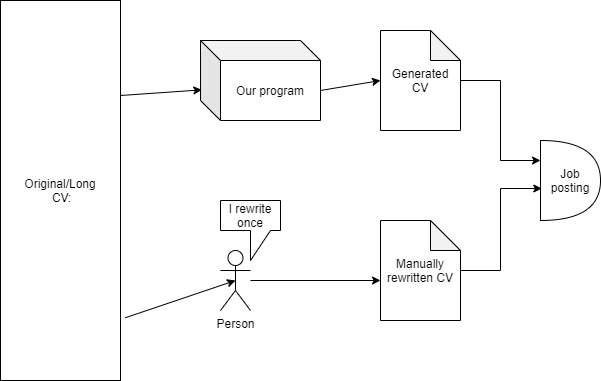
\includegraphics[scale = 0.6]{figures/experiment1.png}
  \caption{Experiment Method}\label{fig:ie}
\end{figure} 
In the experiment, we will create a long CV where all the original information
is in. We do this to ensure that there is no extra information in the human 
rewritten CV that our program couldn't have created. In this way, we ensure
the test is as fair as possible.\\

Thereafter the danish job center will be asked, to answer which of the two CVs is most suited
for the job posting. How this works is as such: \\

The human will shorten down and create a CV based on the long CV. This CV is
is gonna be compared to n number of job postings.
Our program is gonna filter down the long CV, and create a job application,
for each job posting. 
To ensure, that some job postings don't just have lower requirements, we will be
comparing the new CV applications from both the program and the person to the same job postings each time. In total, we will be comparing n number of applications. \\

In this way, we can assume that both the human who had rewritten one
CV and the program, which has rewritten n number of CVs,
will take about the same amount of time, to create n CVs.
Therefore we can somewhat ensure that the results are somewhat fair, concerning the amount of effort each set of n CV's requires.
The structure of both CV's should also remain the same in the testing, such that one CV isn't prioritized because of better formatting.
This is important since the test is primarily testing the CV's contents compared to the job opening. \\

This experiment will compare the results of how many times one gets a "job
interview" using one of the two methods: Comparing the amount of 
"job interviews" (based on what the job center thinks is most likely to earn an interview) 
from the qualitatively created CV from
the human, to the quantitatively created CV from the program to
each other. \\

The results from this will be a good indication, whether our program solved, or
at least helped, in the process of getting a job interview, or if just manually
creating one good application is better.

\subsection{Results}
After we were finished with the program, we decided to print out one CV that has been made by a human,
and 15 almost identical CV to each other the only differences is 
the background information is matching to each keyword there is in the given job posting, 
therefore the text has been custom-tailored to the job posting. \\

We went to the job center to ask a job counselor about which of those 2 CV's were most likely to grant one an interview. \\

She had the following comments:
\begin{itemize}
  \item 1. She thought the overall structure of the human-made CV was better since it was less robotic.
  \item 2. She thought that the contents of the custom made CV, were much more likely to grant one an interview.
  \item 3. She commented on, how the biggest utility of the generated CV, was that it made it a lot easier to include appropriate skills. Since most people have lots of skills but are bad at selecting which to include.
  \item 4. She remarked, that since it was more robotic, it may not catch the recruiter's eye if they are hiring personalities instead of skills.
\end{itemize}

Overall, it can be concluded, that if one wishes to apply a utilitarian and concrete view of one's abilities, then the generated CV is a success.
Though, if one wishes to get a specialized job, where personality and good structure matter a lot, then it may not be advantage to use our CV generator.

\clearpage